% --------------------------------------------------------------------

\textbf{Huomautuksia arvioijalle}

Symbolilla --> merkitsemäni kohdat ovat ideoita sisällöstä. Näiden olisi
kuitenkin tarkoitus kuvata lopullista sisältöä, eli niiden kuuluu olla
loogisessa järjestyksessä ja muutenkin olla järkeviä.

Olen merkinnyt kulmasulkeilla < > viitteet jotka toistaiseksi puuttuu lähteistä.

Olen pyrkinyt muotoilemaan uusiksi kaikki kohdat jossa oli käytetty ensimmäistä
personamuotoa. Sitä ei pitäisi enää esiintyä.

\newpage

\section{Johdanto}

Ohjelmistoalan kilpailutilanteen kiristyessä yritykset etsivät jatkuvasti tapoja
tehostaa toimintaansa. Ketterien menetelmien on todettu parantavan tehokkuutta
sekä laatua \citep{Livermore2008}, mikä nostaa ne houkuttelevaksi vaihtoehdoksi
tehostamista tavoitteleville yrityksille. Ketterien menetelmien käyttöönotto on
kuitenkin haastavaa suurissa yrityksissä \citep{Dyba2009}. Alun perin pieniin
projekteihin ja tiimeihin\footnote{Tässä työssä käytetään ohjelmistoalalla
vakiintunutta lainasanaa tiimi (engl. team) viitaten projektin työryhmään.}
suunnitellut mallit ovat osoittautuneet vaikeiksi soveltaa suuremmassa
mittakaavassa \citep{Boehm2005}.

Suuret yritykset toimivat usein perinteisten ohjelmistotuotannon mallien
mukaisesti. Nämä mallit pyrkivät optimoimaan toimintaa tarkalla suunnittelulla
ja prosessien määrittelyllä. Tämänlainen lähtökohta soveltuu kuitenkin huonosti
ohjelmistokehitykseen, sillä kehitysprojekteissa tulee lähes poikkeuksetta
tilanteita, joita on mahdotonta tai liian työlästä ennustaa \citep{Schwaber2002}.
Suurimpia ongelmia suunnitelmavetoisissa menetelmissä on vaatimusten muuttamisen
korkea hinta sekä myöhäinen palaute tuotteen laadusta \citep{Petersen2010}.
Pitkät julkaisuvälit, muutoksiin vastaamisen kalleus sekä etäisyys asiakkaista
heikentävät yritysten kilpailukykyä. Apua näihin ongelmiin toivotaan löytyvän
ketterien kehitysmallien soveltamisella.

Tämän työn tavoite on esittää nykyinen tutkimuksen tila ketterien
ohjelmistokehitysmenetelmien käyttöönotosta suurissa organisaatioissa,
tarkastellen erityisesti siihen liittyvää organisaatiomuutosta. Ketterien
menetelmien käyttöönotosta on olemassa tutkimuksia, mutta ne keskittyvät
enimmäkseen pieniin organisaatioihin tai yksittäisiin tiimeihin. Suuret
organisaatiot mukautuvat uusiin menetelmiin hitaammin, mikä voidaan olettaa
syyksi siihen, että laajaa tutkimusta suuren mittakaavan ketterästä muutoksesta
ei ole aikaisemmin tehty.

Tämä työ on toteutettu mukaillen järjestelmällisen kirjallisuustutkimuksen
muotoa, kartoittaen olemassa olevat tapaustutkimukset ja kokemusraportit.
Kandidaatintyön laajuudessa järjestelmällisen kirjallisuustutkimuksen menetelmä
tulkitaan kokeelliseksi osuudeksi. Työn tulos osoittaa, että ketterien
kehitysmenetelmien käyttöönotosta isoissa organisaatioissa on olemassa
riittävästi ensisijaisia tutkimuksia kirjallisuustutkimukseen.

\subsection{Tutkimuskysymykset}
Seuraava tutkimuskysymys on asetettu ohjaamaan kirjallisuustutkimuksen
suunnittelua sekä tulosten analysointia:
\textit{Mitkä tekijät vaikuttavat ketterän kehitysmallin organisaatiomuutoksen
läpiviemiseen isossa organisaatiossa?} Tutkimuskysymys on edelleen jaettu
kolmeen alla listattuun alakysymykseen.

\begin{itemize}
\item Miksi organisaatiomuutokseen ryhdytään?
\item Minkälaisia organisaatiomuutoksia on raportoitu?
\item Mitkä ovat muutosprosessin menestyksen ja ongelmien tekijät?
\end{itemize}

\subsection{Työn rajaus}
Kirjallisuustutkimuksessa huomioitavat lähteet on rajattu tutkimusten tyypin,
organisaation koon sekä muutosnäkökulman perusteella. Tutkimustyyppinä on
huomioitu ainoastaan empiirisiä tutkimuksia, eli tapaustutkimuksia, sekä
kokemusraportteja. Tutkitun organisaation tulee olla riittävän iso, jotta
voidaan katsoa ketterien menetelmien suuren mittakaavan haasteiden tulevan
esille \citep{Lindvall2004}. Tutkimukset jotka käsittelevät vain yksittäisiä
tiimejä on rajattu ulos. Organisaatiolla on oltava määritelty aikaisempi
toimintamalli siten, että tutkimuksessa esitetään suunnitelmallinen muutos
ketteriin menetelmiin. Muutoksen lopputilaa tai organisaation uutta
toimintamallia ei ole syytä rajata mihinkään tiettyyn ketterään menetelmään,
sillä käsitykset ketteristä menetelmistä saattavat vaihdella tai muutos olla
vielä kesken.

\subsection{Työn sisältö ja rakenne}
Luvussa \ref{sec:tausta} esitellään aikaisempia tutkimuksia liittyen tämän työn
aihealueeseen, sekä todetaan että työ vastaa olemassa olevaan aukkoon
tutkimuksessa. Luvussa \ref{sec:menetelma} on esitelty järjestelmällisen
kirjallisuustutkimuksen menetelmä, sekä tapa jolla sitä on sovellettu tämän
kandidaatintyön kokeellisena osiona. Luvussa \ref{sec:tulokset} käsitellään
kirjallisuustutkimuksen tulokset. Lopuksi esitellään tuloksista tehdyt
johtopäätökset sekä työn yhteenveto.


% --------------------------------------------------------------------

\section{Työn taustat}
\label{sec:tausta}

Tämän työn tavoitteena on kuvata ketterien kehitysmenetelmien käyttöönoton
perusteita, haasteita ja menestyksen tekijöitä. Näitä tekijöitä tarkastellaan
erityisesti organisaatiomuutoksen näkökulmasta. Taustatietona työlle tässä
luvussa esitellään edellisiä tutkimuksia jotka liittyvät suuren mittakaavan
ketterään kehitykseen, sekä ketterien menetelmien käyttöönotton haasteisiin.
Tämän työn merkitys suhteessa olemassa olevaan tutkimuskeen perustellaan luvun
lopuksi.

\subsection{Ketterä ohjelmistokehitys}
--> Yksi kappale joka summaa ketterän ohjelmistokehityksen pääpointit
(Ketterä ohjelmistokehitys on toki äärettömän laaja alue itsessään, mutta
tämän työn puitteissa siitä ei kannata selittää kuin yksi kappale. Etsin
tähän kaksi viitettä, jotka kuvaavat ketterää kehitystä ylipäänsä)
Boehm,B.: Get ready for agile methods, with care
Highsmith,J.: Agile software development: the business of innovation


\subsection{Aikaisemmat tutkimukset}

--> Dybån ja Dingsøyrin tutkimuksen lisäksi tehtiin haku ketterien menetelmien
käyttöönottoa tai suuren mittakaavan soveltamista kuvaavista tutkimuksista.
--> löytyi 5 kappaletta aikaväliltä 2004-2009
--> Nämä ovat tämän tutkimuksen aihealueeseen vahvasti liittyviä
--> Alla on esitelty erityishuomioita kustakin tutkimuksesta

\cite{Dyba2008} ovat julkaisseet ainoan laajan ja järjestelmällisen
kirjallisuustutkimuksen joka yleisellä tasolla tarkastelee ketterää
ohjelmistokehitykstä. Tutkimuksen tuloksena todettiin muun muassa, että ketteriä
menetelmiä on vaikea soveltaa isommassa mittakaavassa kuin ''pienet tiimit''.
--> 7 tutkimusta 36 käsittelivät ketterän menetelmän käyttöönottoa.
--> Extreme Programming oli lähes ainoa menetelmä josta oli tehty tutkimusta.
--> Tutkimuksen tekijät suosittelivat suositun Scrum-menetelmän tutkimista.
\citep{Dyba2008}

\citep{Lindvall2004}:
--> Kvalitatiivista dataa neljästä organisaatiosta. \newline
--> Suurten organisaatioiden erityispiirre on tiimienvälisen koordinoinnin
tarve. Koordinoinnin takia tiimien on välttämättä tuotettava lisää
dokumentaatiota ja pidettävä kokouksia toisten tiimien kanssa, mikä vähentää
ketteryyttä. \newline
--> Ketterät menetelmät saattavat joutua törmäyskurssille organisaation olemassa
olevien toimintojen kuten muutoslautakunnan (engl. change control board) kanssa. \newline
--> Organisatorilliset prosessit

\citep{Nerur2005}:
--> On ymmärrettävä että uuden menetelmän käyttöönotto aiheuttaa muutoksia koko
organisaation laajuisesti. \newline
--> Organisaatiokulttuuri on uudistettava, sillä vanhat toimintatavat ovat usein
syvälle juurtuneita. \newline
--> Toimintatapojen on muututtava ihmislähtöisiksi. \newline
--> Tuotantoprosessin on muututtava elinkaarimallista tukemaan
ominaisuuspohjaista (engl. feature-based) kehitystä. \newline
--> Uusiin työkaluihin on panostettava sekä hankintakustannuksia että
käyttöönoton vaatima työ.

\citep{Boehm2005}:
--> Konfliktit kehitysprosessissa: Kehitysprosessin muutokseen pitää
valmistautua huolella, ja prosessi pitää rakentaa alhaalta ylös. \newline
--> Liiketoimintaprosessien knofliktit: Liiketoiminnan johdon on hyväksyttävä
että tarkoilla aika- ja kustannusarvioilla ei ole sijaa ohjelmistokehityksessä.
Myös sopimuskäytännöt pitää uusia, mikä saattaa vaatia neuvotteluja asiakkaan
kanssa. \newline
--> Ihmislähtöisyys on kettrien menetelmien lähtökohta. Ihmisten välinen
interaktio on avaintekijä ketterässä kehityksessä. Tämä on huomioitava
johtamisen tyylissä, joka on perinteisissä organisaatioissa usein määräävä. On
myös oletettavaa että osa henkilöstöstä ei halua muuttaa toimintatapojaan.
Näiden haasteiden selvittäminen vaatii henkilöstön kouluttamista, sekä
ymmärrystä siitä miten ihmisten väliset interaktiot luovat sujuvaa
kommunikaatiota.

\citep{Livermore2008}:
--> Verkossa toteutettu kyselytutkimus, joka kartoitti mitkä tekijät korreloivat
ketterien menetelmien menestyneen käyttöönoton kanssa. \newline
--> Uudet menetelmät vaativat koulutusta -- koulutus oli merkittävä tekijä. \newline
--> Johdon tuki korreloi vahvasti \newline
--> Tarkan muutossuunnitelman laatiminen ei vaikuttanut olevan menestyksen tekijä \newline
--> Ulkopuolisen avun käyttäminen, esimerkiksi konsulttien, oli vahvasti
kytköksissä menestyksekkääseen muutokseen. \newline
--> Muutokset olivat onnistuneet pienissä organisaatioissa, kun taas suurilla
organisaatioilla oli ollut vaikeuksia. \newline
--> Johtopäätöksenä: pitää varata tarpeeksi resursseja muutosta varten.

\citep{Misra2009}:
--> Suuren mittakaavan kyselytutkimus. \newline
--> Määräävän ja määriteltyihin käytäntöihin perustuvan organisaatiokulttuurin
on muututtava sallimaan vapaus valita toimintatavat ja hajautettu johtaminen.
Organisaation on myös muututtava asiakaskeskeiseksi. \newline
--> Johtamistyylin on muututtava avoimemmaksi ja muutoksia sallivammaksi. Johdon
on hyväksyttävä riskien ja epävarmuuden olemassaolo, ja luotettava kehittäjiin.
Raportoinnin on perustuttava rehellisyyteen ja läpinäkyvyyteen, ja projektien
tila on esitettävä avoimesti. \newline 
--> Kehitysprosessin syklit on muutettava lyhyiksi ja kehityksessä on sallittava
muutoksia. \newline
--> Koko henkilöstöä on koulutettava ketterien mallien käytöstä ja periaatteista.
Erityisesti johdon kouluttaminen on tärkeää. \newline
--> Esitetyillä tekijöillä ei ollut keskeistä prioriteettia, jota tutkimuksessa
haettiin, vaan kaikki tekijät vaikuttavat yhtä tärkeiltä muutoksen kannalta

Mahanti, Aniket: Challenges in Enterprise Adoption of Agile Methods - A Survey

\subsection{Yhteenveto aikaisemmista tutkimuksista}

--> Tärkeimmät teemat yhteenvetona. Jos pystyy petaamaan pohjaa tulosten
keskeisimmistä havainnoista, niin hyvä.

--> Organisaatiokulttuurin muuttaminen \newline
--> Koulutus

% Tässä oli ennen ''työn motivointi'', eli tutkimusaukon määrittely
\subsection{Uuden tutkimuksen tarve}
Kuten yllä havattiin, ketteristä menetelmien soveltamisesta on julkaistu useita
aikaisempia tutkimuksia. Myös suuren mittakaavan ketterästä kehityksestä on
tutkimuksia, kuten myös ketterien menetelminen käyttöönottoon liittyvästä
organisaatiomuutoksesta. Suureen mittakaavaan tai organisaatiomuutokseen
liittyvät tutkimukset ovat enimmäkseen olleet primääritkimuksia, mukaan lukien
tapaustutkimuksia sekä kokemuskertomuksia. Laajaa kirjallisuustutkimiusta
keterän kehitysmallin käyttöönottoon liittyvään organisaatiomuutokseen ei ole
tehty. Näin ollen nykyiset julkaisut jättävät selkeän aukon yhteenvetävälle
kartoitukselle raportoiduista havainnoista suuren mittakaavan ketterässä
kehityksessä.

% --------------------------------------------------------------------

\section{Tutkimusmenetelmä}
\label{sec:menetelma}

Tässä luvussa esitellään työssä käytetty järjestelmällisen
kirjallisuuskatsauksen tutkimusmenetelmä. Ensiksi esitellään menetelmän
periaatteet, ja kuvataan miten sitä on mukautettu soveltumaan kandidaatintyöhön.
Tämän jälkeen esitellään menetelmän vaiheiden suorittaminen kandidaatintyön
kokeellisena osiona.

\subsection{Järjestelmällisen kirjallisuustutkimuksen menetelmä}

Tässä työssä käytetty tutkimusmenetelmä myötäilee Kitchenhamin esittämää mallia
ohjelmistotuotannon alan kirjallisuustutkimukseen. Valitun menetelmän tavoite on
muodostaa yhtenäinen kuva tämänhetkisestä tutkimuksesta työn aihealueella.
Ohjelmistotuotannon alan kirjallisuustutkimus suoritetaan pääasiallisesti
tekemällä hakuja elektronisiin tietokantoihin ja arvioimalla hakujen perusteella
löytynyttä aineistoa. Kirjallisuustutkimuks sisältää viisi pääasiallista
vaihetta: hakujen suunnittelu, aineiston seulonta, aineiston laadun arviointi,
tiedon poiminta sekä synteesin tekeminen. \citep{Kitchenham2007}

Järjestelmällisen kirjallisuustutkimukseen kuuluu lisäksi ulkopuolinen
katselmointi ja systemaattinen tutkimusprotokollan seuraaminen
\citep{Kitchenham2007}, mutta niiden soveltaminen ylittää kandidaatintyön
laajuuden.

\subsection{Hakujen suunnittelu}
Hakujen suunnittelulla tarkoitetaan käytettävien elektronisten aineistojen
valintaa ja hakulausekkeiden muodostamista. Elektronisina aineistoina käytettiin
seuraavia ohjelmistotuotannon alan julkaisuja hyvin kattavia tietokantoja:
IEEExplore <link>, ACM <link>, Scopus (ScienceDirect??) <link>, ProQuest <link>.
Näiden lisäksi suoritin haun <XP~Conference> arkistoon.

Ennen varsinaisten hakujen suorittamista suoritettiin esihakuja. Näiden
tarkoituksena oli kartoittaa hyviä avainsanoja varsinaisiin hakuihin. Esihauissa
käytettiin muun muassa termejä \textit{agile transformation} sekä \textit{large
scale agile}. Esihakujen perusteella löytyi useita aihealueeseen liittyviä
tutkimuksia.

Varsinaisissa hauissa käytettävät hakulausekkeet ovat boolen logiikalla
muodostettavia lausekkeita, jotka määräävät avainsanat joiden tulee esiintyä
hakutuloksissa. Hakulusekkeita varten määrittellään joukko näkökulmia jotka
edustavat tutkimuskysymysten aihepiiriä. Jokaista näkökulmaa kohden etsitään
yleisimmin käytettyjä avainsanoja sekä niiden synonyymejä. Lopuksi
hakulausekkeet muunnetaan boolen lausekkeiksi käyttämällä
\texttt{OR}-operattoria avainsanojen välillä, sekä \texttt{AND}-operaattoria
näkökulmien välillä. Taulukko~\ref{table:hakulausekkeet} esittää tässä työssä
käytetyt näkökulmat ja niitä vastaavat avainsanat.

\begin{table}[h]
    \begin{tabular}{|l|l|}
        \hline
        Näkökulma           & Avainsanat   \\ \hline
        Ketterät menetelmät & agile, scrum, lean, xp \\ 
        Organisaatiomuutos  & transformation, transition, change, migration \\
        Suuri organisaatio  & enterprise, organization, (large \texttt{AND} scale) \\
        \hline
    \end{tabular}
	\caption{Hauissa käytetyt näkökulmat ja niitä vastaavat avainsanat}
	\label{table:hakulausekkeet}
\end{table}

Kaikkia esihaun viitteitä ei löytynyt varsinaisessa haussa. Tämä johtuu siitä,
että osa tiivistelmistä on epäinformatiivisia, eivätkä sisällä avainsanoja.
Jotkut viitteet ovat myös otsikoitu epämääräisesti tai kekseliäästi, jonka takia
täsmällinen hakulausekke ei löydä niitä. Esihekujen löytämät viitteet olivat
kuitenkin selkeästi oleellisia, joten ne on liitetty varsinaisilla hauilla
kerättyyn aineistoon.

\subsection{Aineiston seulonta}

Kun suunnitellut haut on suoritettu on koottujen viitteiden joukosta seulottava
ne tutkimukset jotka ovat oleellisia kirjallisuustutkimuksen kannalta. Tämän
työn puitteissa seulonta suoritettiin kahdella tasolla: ensiksi otsikon
perusteella, ja sitten tiivistelmän perusteella. Otsikon perusteella hylättiin
vain selkeästi aihealueeseen kuulumattomat lähteet, sillä useat oleellisilta
vaikuttavat työt olivat otsikoitu epäselvästi. Otsikon perusteella valittiin 117
lähdettä. Tiivistelmän perusteella lähteet arvioitiin kolmesta näkökulmasta:
ketterä ohjelmistokehitys, suuri organisaatio tai monta tiimiä ja
toimintatapojen muutos. Tarkempaan tarkasteluun valittiin vain ne lähteet jotka
tiivistelmän perusteella käsitelivät kaikkia kolmea näkökulmaa. Tällä
menetelmällä tarkempaan tarkasteluun valittiin 31 lähdettä. Valituista lähteistä
yksi ei ollut saatavilla, jolloin tiedon poiminta suoritettiin lopulta 30
lähteelle.

\subsection{Tiedon poiminta}

Valitut ensisijaiset tutkimukset arvioidaan poimimalla niistä oleelliset tiedot.
Tiedon poimintaan käytetään tiedonkeruulomaketta, joka täytetään kutakin
tarkempaan tarkasteluun valittua lähdettä kohden. Tämän työn
tiedonkeruulomakkeessa käytettiin taulukossa \ref{table:dataform} listattuja
kenttiä.

\begin{table}[h]
    \begin{tabular}{|l|l|}
        \hline
        Transformation mentioned in text (Y/N) &
        Large scale mentioned in text (Y/N) \\
        Is empirical case study (Y/N) &
        Is industry experience report (Y/N) \\
        Has listing of practices (Y/N) &
        Used research method (Y/N) \\
        Relevance to this review (1-5) & \\
        Objective of research (or publication) &
        Research method \\
        Author bias &
        Validity threats \\
        Organization size &
        Time of transformation \\
        Initial state of organization &
        Why was the change initiated \\
        How was the change conducted &
        What is agility? / Which agile paractices are used? \\
        Findings / lessons learned &
        Good practices validated or suggested by study \\
        Reported challenges &
        Satisfaction after transformation \\
        Effect on organization &
        Measurements as results (quantitative or other) \\
        Other notes &
        Notable references \\
        \hline
    \end{tabular}
    \caption{Työssä käytetyt tiedonkeruulomakkeen kentät. Kentät merkinnällä
    (Y/N) ovat kyllä/ei muotoisia kenttiä. Kentät merkinnällä (1-5) ovat
    pisteasteikon muodossa olevia kenttiä. Muut kentät ovat vapaamuotoisia
    tekstikenttiä.}
    \label{table:dataform}
\end{table}


% --------------------------------------------------------------------

\section{Tulokset}
\label{sec:tulokset}

Tässä luvussa esitellään synteesi ensisijaisista tutkimuksista ja raporteista
poimituista tiedoista. Lähteiden keruu ja tietojen poiminta on suoritettu
myötäillen luvussa \ref{sec:menetelma} esitetyä Kitchenhamin
kirjallisuustutkimuksen menetelmää \citep{Kitchenham2007}. Luvun alussa
esitellään yhteenveto tutkimuksista joita tarkasteltiin. Tämän jälkeen annetaan
yleiskatsaus tutkimuksissa kuvatuista ketteristä menetelmistä. Luvun loppuosa
käsittelee tutkimuskysymyksiin liittyvät oleellisimmat havainnot.

\subsection{Yhteenveto tutkimuksista}

Tutkitusta materiaalista 23 kappaletta oli teollisuuden kokemusraportteja, ja 7
kappaletta oli tapaustutkimuksia. Suurin osa julkaisuista oli
konferenssijulkaisuja, ja aineisto sisälsi vain kolme lehtiartikkelia. Tulosten
kannalta on tärkeä huomioida että suurin osa julkaisuista oli yritysten
työntekijoiden laatimia kokemusraportteja. Tämä seikkan valossa tuloksiin on
suhtauduttava varauksella. Erityisesti raportoituihin ongelmiin (tai niiden
puuttumiseen) ja positiivisiin tuloksiin on suhtauduttava varauksella.

Kuten kuva~\ref{fig:publications} näyttää, kaikki valitut tutkimukset olivat
julkaistu noin kymmenen vuoden sisällä. Tutkittu materiaali esittää nousun
ketterien menetelmien suosiossa vuoden 2007 kohdalla, mutta julkaisuiden
lukumäärä vaikuttaa pysyvän tasaisena. Huomattavaa on, että
organisaatiomuutoksia on raportoitu heti vuosituhannen vaihteen jälkeen, jolloin
ketterät menetelmät alkoivat tulla tunnetuksi. Tästä voidaan vetää johtopäätös,
että suuret yritykset ovat olleet kiinnostuneita ketterien menetelmien
soveltamisesta hyvin pian niiden esittelemisen jälkeen.

\begin{figure}[htb]
  \begin{center}
    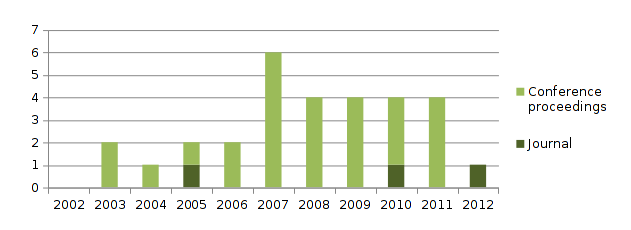
\includegraphics[width=1\textwidth]{img/Publications}
    \caption{Julkaistut tutkimukset vuosittain}
    \label{fig:publications}
  \end{center}
\end{figure}

Suurimmassa osassa julkaisuja oli ilmoitettu ajankohta jolloin muutoksen ensi
askeleet oli otettu. Kuva~\ref{fig:start_year} esittää ilmoitetut muutosten
alkuajankohdat ryhmiteltynä vuosittain. Mediaani muutoksen aloitusajankohdasta
julkaisuvuoteen oli kolme vuotta. Tämä näkyy verrattavasti julkaisujen kasvun
nousussa vuonna 2007 ja aloitettujen muutoshankkeiden nousussa vuonna 2004.
Tästä voidaan päätellä että suuren mittakaavan muutokset ketteriin menetelmiin
ovat yleistyneet viime vuosikymmenen puolesta välistä alkaen. 

\begin{figure}[htb]
  \begin{center}
    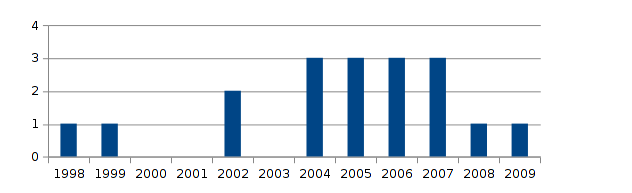
\includegraphics[width=1\textwidth]{img/Transformation_start}
    \caption{Organisaatiomuutosten aloitusajankohdat vuosittain}
    \label{fig:start_year}
  \end{center}
\end{figure}

\subsection{Käytetyt ketterät menetelmät}

Kaikkissa tapauksissa organisaatio oli päätynyt jatkamaan ketterän mallin
käyttämistä. Muutoksen vaikutuksia oli tyypillisesti raportoitu 1 tai 2 vuoden
päähän sen aloittamisesta. Suurimmassa osasta tapauksia muutos katsottiin
edelleen jatkuvan raportin kirjoitusajankohtana.

Suurin osa tutkimuksta erotteli käytössä olevia ketteriä menetelmiä.
Taulukko~\ref{table:practices} esittää tutkimuksissa eniten raportoidut
menetelmät. Ylivoimaisesti suosituin ketterä menetelmä oli Scrum, jota
mainittiin käytettävän miltei kahdessa kolmesta organisaatiosta. Toiseksi
suosituin menetelmä oli Extreme Programming (XP). Osassa organisaatioista myös
kevyt kehitysmalli (engl. lean development) oli yhdistetty ketteriin
menetelmiin.

Taulukosta~\ref{table:practices} ilmenee myös eri menetelmien yhdistely
huomattavana trendinä. Lähes kolmanneksessa raporteista mainittiin suoraan, että
menetelmiä oli yhdistelty. Menetelmien yhdistelemistä ja räätälöintiä oli
perusteltu pääasiallisesti kahdella tapaa. Osassa raporteista oli syyksi
mainittu se, että suuren organisaation erityispiirteet tekivät menetelmän
räätälöinnin välttämättömäksi. Toisaalta yritykset olivat halunneet panostaa
mahdollisimman hyvän menetelmän löytämiseen, jolloin useita menetelmiä oli
arvioitu ja niiden sopivimmat piirteet oli yhdistetty.

\begin{table}[h]
    \begin{tabular}{|l|l|}
        \hline
        Menetelmä       & N   \\ \hline
        Scrum           & 18 \\ 
        XP              & 7 \\
        Lean            & 5 \\
        Eri menetelmien yhdistely ja räätälöinti & 9  (epäsuorasti mainittuna useampia) \\
        \hline
    \end{tabular}
	\caption{Hauissa käytetyt näkökulmat ja niitä vastaavat avainsanat. Sarake N
	kuvaa kuinka monessa tutkimuksessa menetelmää mainittiin käytettävän.}
	\label{table:practices}
\end{table}

Edellä mainittujen ketterien mallien lisäksi oli yksittäisiä mainintoja
seuraavista menetelmistä: JAD (Joint Application Development),
ASSF\footnote{Katso Qumer \& Henderson-Sellers 2007}, Unified Process, sekä DSDM
(Dynamic Systems Development Method). Näiden menetelmien lisäksi mainittiin
erilaisia käytäntöjä mukaan lukien ajallinen rytmittäminen (engl. time-boxing),
testivetoinen kehitys, asiakkaan mukanaolo, testauksen automatisointi, sekä
jatkuva yhdentäminen (engl. continuous integration).

\subsection{Tutkimuskysymyksiin liittyvät havainnot}

\textbf{Miksi organisaatiomuutokseen ryhdytään?}

\textbf{Minkälaisia organisaatiomuutoksia on raportoitu?}

\textbf{Mitkä ovat muutosprosessin menestyksen ja ongelmien tekijät?}

\vspace{1cm}
\textbf{Muuta}

--> Viitteiden validiteetti (kuinka suuri luottamus)

% --------------------------------------------------------------------

\section{Johtopäätökset ja yhteenveto}
\label{sec:johtopaatokset}

--> Muistutus työon tavoitteista (sidoksisuus johdantoon)

--> Yhteenveto tuloksista, ja tulosten merkitys
--> Suositus toimnepiteisiin??

--> Tulosten soveltuvuus
--> Tutkimuksen arviointi

--> Lisätutkimuskysymyksiä jatkoa varten: käyttöönoton laajuus /
oerganisaatiotyypit / mitkä menetelmät / enemmän perusteita miksi ?? 

--> Jatkotutkimukset
--> Pitää tehdä kirjallisuustutkimus seuraten huolellisesti jotakin
kijallisuustutkimuksen menetelmää. Jotta sain järjestelmällisen
kirjallisuustutkimuksen sovitettua kandidaatintyön laajuuteen jouduin
karsimaan useita oleellisia menetelmään kuuluvia muodollisuuksia.


